\documentclass{umm-senior-sem}
\usepackage{cite}
\usepackage{url}

%\usepackage{setspace}
%\setstretch{2} 
\begin{document}
\title{Summary of Using Ant Colony Optimizations to Learn Fuzzy Cognitive Maps}
\author{
\alignauthor
Chris Aga \\
\affaddr{ 
University of Minnesota, Morris \\
600 East 4th St. \\	
Morris, Minnesota 56267} \\
\email{agaxx010@morris.umn.edu}
}

\maketitle

\begin{abstract}
This paper summarizes the application of Ant Colony Optimizations (ACO) to model accurate relationships between multiple concepts in a system when expert knowledge is lacking. The model used in~\cite{main:2012} by Ye Chen is termed Fuzzy Cognitive Map. It consitsts of nodes (concepts) with weighted edges which represent the magnitude of exhibition or inhibition of all concepts towards each other. Chen gives a brief summary on FCMs, approaches to learning of FCMs and compares their efficiencies to one another. The approach discussed in depth for learning of FCMs in~\cite{main:2012} was ACO. This paper attempts to explain in more accurate detail each of the concepts covered in Chen's paper.
\end{abstract}

\keywords{Fuzzy Cognitive Maps, Ant Colony Optimization, numerical optimization, data-driven learning algorithm}

\section{Introduction}
\label{sec:intro}
Accurate models of relationships and interactions between genes in a cell can be hard to generate due to lack of expert knowledge. Typically, a passable amount of knowledge is available on determining relationships between concepts such as genes in a cell, Fuzzy Cognitive Maps (FCM) are a common model used to represent these relationships because of their readability and ability to handle logic in a approximated form. Typically, enough expert knowledge is known to generate a tolerable FCM, and from there, a learning technique is used to improve the accuracy of an FCM. Even though a large abundance of data on the particular state of genes at many moments are available, without proper knowledge, developing accurate causal relationships between each concept is nontrivial. This is where the learning of FCMs with randomly generated relationships between concepts is important. Ye Chen in~\cite{main:2012} investigates the use of Ant Colony Optimizations (ACO) as a solution to this problem. 

The following section will give a brief overview of what a Fuzzy Cognitive Map is, describe the purpose of ``learning'' a Fuzzy Cognitive Map and comment on current learning approaches. The model of Ant Colony Optimizations and its application to the learning of Fuzzy Cognitive Maps will be explained in depth in Section~\ref{sec:aco}. Finally, Section~\ref{sec:comparison} will compare the previously discussed learning approaches to Ant Colony Optimization as a learning approach.

\begin{figure}
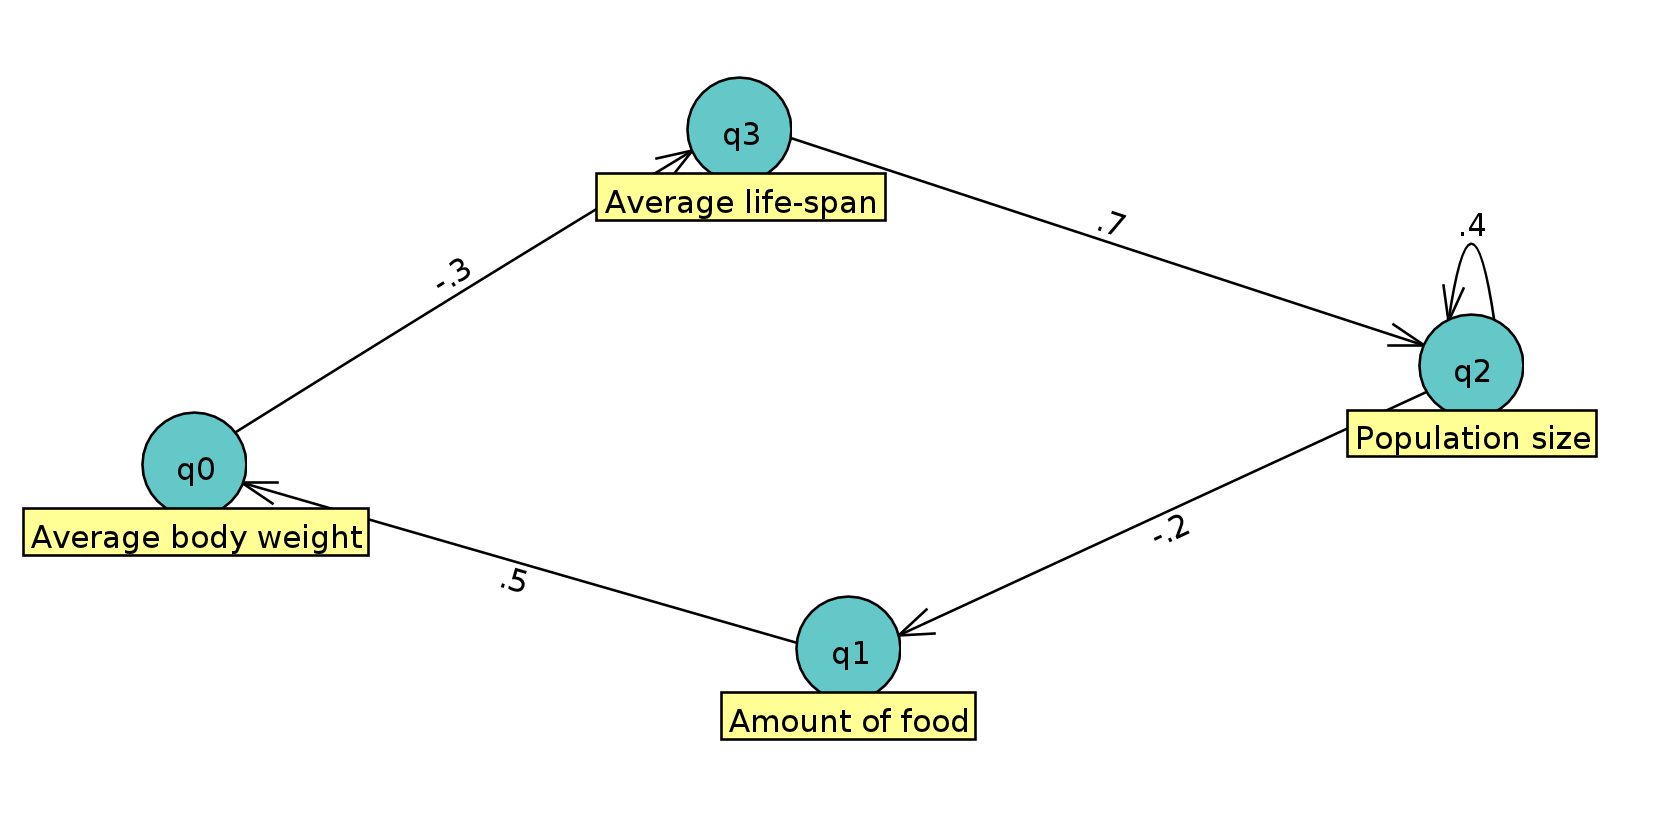
\includegraphics[width = 8cm, height = 4cm]{images/population.png}
\label{fig:fcm}
\caption{Example of a Fuzzy Cognitive Map representing concepts that affect each other among a population of people (figure created in JFlap)}
\end{figure}

\section{Learning of Fuzzy Cognitive Maps}
\label{fcm}
\subsection{Fuzzy Cognitive Maps Background}
A Fuzzy Cognitive Map (FCM) is an object which represents real valued causal relationships (represented by a weighted edge) between concepts (nodes) in a system. An example is depicted in Figure~\ref{fig:fcm} and describes the relationships that: life-span, average body weight, amount of food present among a population, and population-size have with each other. 

FCMs in a very general sense attempt to discover the ``what if'' value of each concept when concepts are affected from input data~\cite{FCMbg:1999}. This is described by the activation degree of a concept which is calculated by taking the sum of each concepts' current value, multiplied by its weight edge pointing towards the concept we're attempting to find the activation degree of. The activation degree is finally calculated by applying a sigmoid function, Equation~\ref{eq:sig}, where $\lambda$ represents a user-defined parameter to ``characterize the steepness of the function around zero''~\cite{main:2012}, to the summation. This value is then saved to the node, this occurs for each node simultaneously.
\begin{equation}
\label{eq:sig}
 f \big(x\big) = \frac{1}{1+ e^{-\lambda x} } 
\end{equation}

\subsection{Concept of learning and its Importance}
The idea of ``learning'' in an FCM attempts to improve either an FCM generated with some expert knowledge backing, or a randomly generated FCM. By the end of the learning process, at each interval, the FCM should be able to output very similar outputs to the data it was learned with. This paper summarizes 2 techniques used for learning, and gives an in depth explination of a third approach termed Ant Colony Optimization (ACO). 

\subsection{Current techniques used for FCM learning}
A major approach used for learning of Fuzzy Cognitive Maps is termed nonlinear Hebbian learning. This model approaches learning in a similarly to how neurons interact and activate during learning in the brain~\cite{response:2003}. Hebbian learning is based on synchronous firing of neurons, neurons (represented as concepts in this system) next to each other directly affect one another. If two concepts are activated simultaneously, this represents the strengthening relationship between two concepts, which is analagous to neural plasticity in the brain. Stach explains in~\cite{nhl:2008} that updating weights of one concept with respect to another when a ``neuron'' fires is best approached by applying the product of the adjacent concepts' weights to one another. A pitfall in this approach is the possibility of reaching infinite growth, but a forgetting term is used to keep the weights in the predefined bounds. 

Another common approach, termed Real Coded Genetic Algorithm (RCGA) is a Genetic Algorithm approach using real numbers to minimize the error of an FCM's output compared to the actual output data used to learn the FCM.

\section{Ant Colony Optimizations}
\label{sec:aco}
Ant Colony Optimization (ACO) is a technique based off of the behaviour of ants attempting to gather food to bring back to their anthill~\cite{main:2012}. When ants look for food, they leave pheromone trails behind and the more a path is traveled, the greater amount of pheromone will be left behind. Shorter paths will be traveled more by a single ant, thus it will have more opportunities to leave behind pheromones, so over time, ants will discover various shortest paths between food sources and their home. This concept is applied to the learning of Fuzzy Concept Maps (FCM) by atttempting to minimize the error between the generated output of an FCM and the actual output data that was used to initially learn the FCM. 
\subsection{Ant tours and activation degree}
\label{sec:activation}
Each ant in the population takes what is called a ``tour'', this involves travelling from each node, to every other node (self inclusive) in the system of concepts. The entire tour represents an ant traveling from its home to a food source. This tour is constructed from various ``checkpoints''. These checkpoints are values that represent the weight of one node to the next. Again, the entire tour an ant takes is of the form: 
\begin{equation}
 \big\{w_{11}, w_{12}, w_{13} ... w_{n,n}\big\} 
\end{equation}
Where each $w_{ij}$ represents the weight from $Concept_i$ to $Concept_j$.
Between each node, there are $N_d$ checkpoints, where $N_d$ is the desired precision of the weighted edge between concepts. Each checkpoint, as depicted in Figure~\ref{fig:antPath}, is a number 0-9, and between each number in a $column_i$ and every other box in the following $column_{i+1}$, a pheromone intensity is present to help guide ants along ``shorter trails'', or in the case of optimizing the accuracy of causality relationships between concepts in an FCM, reducing the difference between FCM concept activation values and actual values of the output data used to generate the FCM. 
\begin{figure}
\label{fig:antPath}
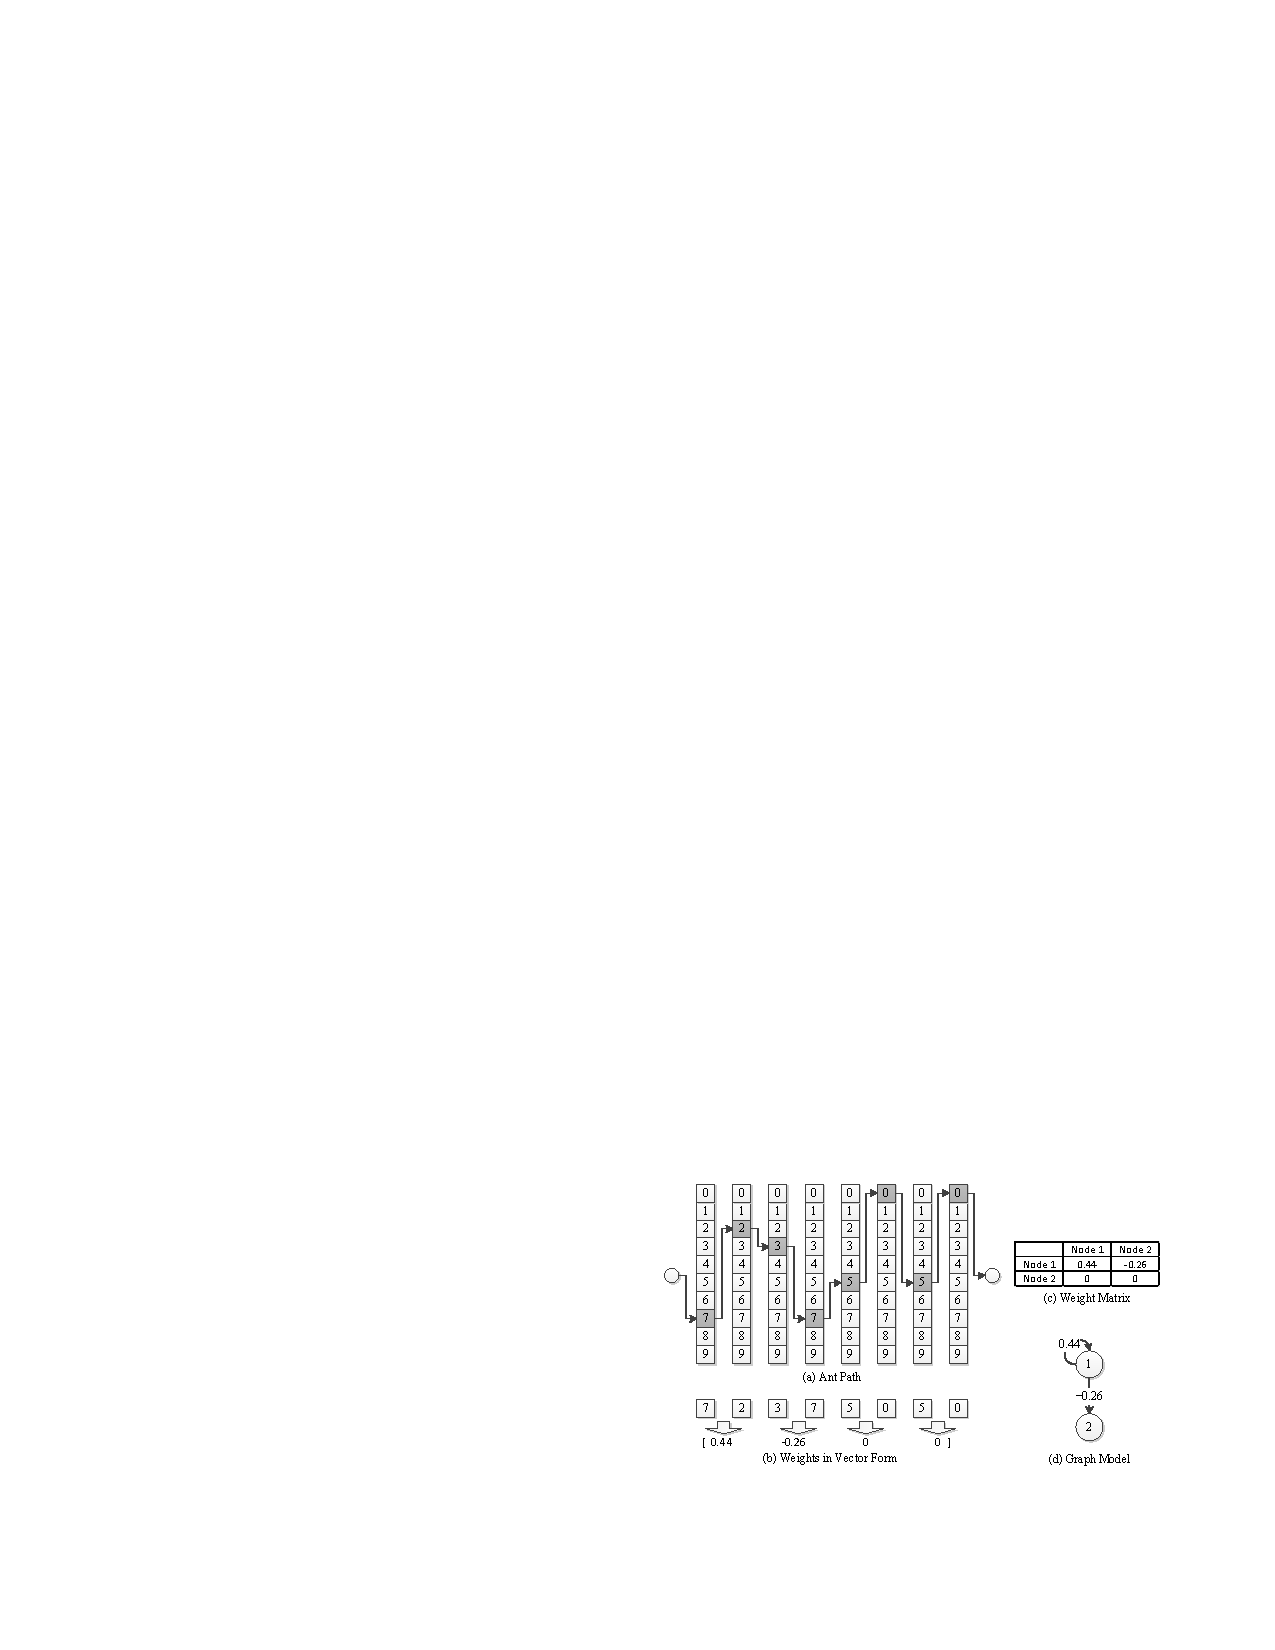
\includegraphics[scale=1]{images/antPath.pdf}
\caption{Figure depicting an ant's path taken (generates a weighted edge for each node) among each node, b represents the vector form, c the weight matrix generated by the weight vector in b, and d depicts the outputted FCM~\cite{main:2012}}
\end{figure}
For example, using precision two for edge weights, and in a system with just two nodes, the path from each node to each other node (again, self inclusive) in the system are represented in Figure~\ref{fig:antPath}a.


For each $ant_i$, after traveling from one checkpoint to the next, locally, the pheromone trail is decayed to encourage $ant_i$ to travel different checkpoint paths. This does not affect the pheromone trail viewed by other ants though. The first tour of all nodes is completely random for each ant, none of the pheromone trails are decayed in the initial run. After all ants have completed the first tour, an FCM is generated for each ant based on its travelled path. Equation~\ref{eq:pathToFCM} is used to transform each vector representation of checkpoints traveled between two nodes to generate a weighted edge between the actual concepts in the FCM. For exapmle,  in Figure~\ref{fig:antPath}, from $column_3$ -> $column_4$ (representing $Node_1$ -> $Node_2$), checkpoints 3->4 were travelled, the weight vector is 0.34 and is respectively transformed via Equation~\ref{eq:pathToFCM} to -0.26,  and is assigned to its respected edge.
\begin{equation}
\label{eq:pathToFCM}
g\big(x\big) = 2 \big(x-0.5\big) 
\end{equation}
\subsection{Global Pheromone Update}
\label{sec:global}
After FCMs have been generated for all ants, the amount of error is evaluated at the current set of output data to determine how accurate an FCM is as a representation for the relationships between all the concepts. For all concepts in the system, $concept_i$'s new activation value is generated based on the approach described in~\ref{sec:activation}, the difference is calculated between this new value and the actual output for $concept_i$ in the output data to determine the amount of error of a concept at a particular point. All these errors are summed up to generate the overall \textit{Data Error} for an entire sequence of data. The ant who generated an FCM with the smallest \textit{Data Error} is deemed most fit and it globally updates the pheromone intensities of particular checkpoints for all ants in the population based on the path that it took. This process is continued for a specifed number of iterations and at the end, a more optimal solution will have been discovered~\cite{main:2012}.

\section{Comparison of Fuzzy Cognitive Map Learning Approaches}
\label{sec:comparison}
Five performance measures were used in the experiment in~\cite{main:2012} to determine how well an FCM was learned via each of the following three techniques: Real Coded Genetic Algorithm (RCGA), Non-linear Hebbian Learning (NHL) and finally ACO. A prior approach to applying ACO to FCM learning was included in the experiment to see if this implementation of ACO outperforms its ancestor.

The first was a model error which tested against a set of data that was, with high certainty to be proper estimates for an FCM that would sufficiently represent the system. The same type of error calculations as used to approximate how fit an ant's generated FCM was used to determine a model's error. Next, a binary transformation was applied to the absolute value of all weights. If they surpassed a user-defined threshold, the weight was set to one, otherwise the edge's value was defaulted to zero. This binary representation was used to calculate the sensitivity, specificity, and a mean representation of the accuracy for each FCM. 

The results of all performance measures found that with a small-scale system of about 5 concept nodes, the ACO outperformed both RCGA and NHL. Although once the amount of concept nodes in the system was increased, for the ACO to do better or keep up, it required more recorded data to be applied to the its learning process. Also, the ACO application to learning an FCM was able to successfully learn 1600 weights on an FCM accurately whereas the prior implantation of ACO that Chen discussed briefly in his paper could only achieve accurate learning of up to 8 weights.
\section{Conclusion}
\label{sec:Conclusion}
When expert knowledge in a field is lacking and a model to represent the causal relationships of concepts are desired, learning of a Fuzzy Cognitive Map via ACO appears to work quite well. The ACO outperformed many of the other learning approaches at lower numbers of concepts but needed more data to outperform them at higher amounts of concepts. 

This implementation was found to significantly outperform a previous application of ACO to learning of Fuzzy Cognitive Maps. Although, as Chen states in~\cite{main:2012}, additions such as ``local search procedures'' could greatly improve the results of FCM learning via ACO, so this approach still has future work to be implemented.

\nocite{*}
%^this is a very important addition so that
%references will be included property

\bibliography{Bibliography}
\bibliographystyle{abbrv}
\end{document}